\chapter{Event Selection}

The subject of this thesis is to study the effect of domain adaptation methods on flavor tagging algorithms to improve the data to simulation agreement. In section \ref{sec:ch_4_da} two domain adaptation methods were introduced. Both have the goal to transfer the source domain and the target domain into a domain invariant feature space that the classifier output becomes domain invariant. To achieve this goals, the source and the target distribution of their input features have to be similar. Furthermore, both domains should have the same distributions in their class compositions. Which means in this case they need to have the same amount of jets each quark flavor in data and simulation. In order to meet these requirements, an event selection is needed. \\

The event selection has several requirements to fulfill. It has to be performed in the same way for data and simulation and the data to simulation agreement for the selected events shall be as good as possible. The mismodeling of the simulation of the jets shall be the dominant reason for the domain discrepancy. The event selection has to be independent of the specific jets in each event. Moreover the selected events should contain balanced fractions of jets of the different categories used in the classifier. Finally the amount of jets should be high enough that the statistical uncertainties are negligible. The last two points are in direct conflict as categories like bb occur mostly for high \pt jets of which not many exist. Therefore the demand of balanced fractions is secondary. 

\section{Top Quark Decay}

\begin{figure}
\hfill
\subfigure[]{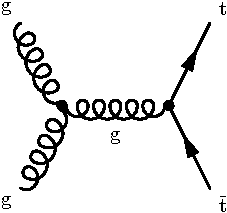
\includegraphics[width=3cm]{assets/Feynman/tt_gg_s.pdf}}
\hfill
\subfigure[]{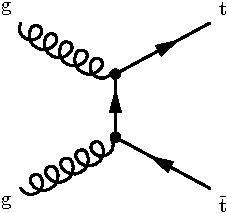
\includegraphics[width=3cm]{assets/Feynman/tt_gg_t.pdf}}
\hfill
\subfigure[]{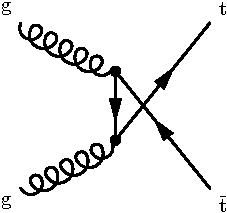
\includegraphics[width=3cm]{assets/Feynman/tt_gg_u.pdf}}
\hfill
\subfigure[]{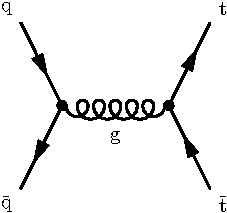
\includegraphics[width=3cm]{assets/Feynman/tt_qq_s.pdf}}
\hfill
\caption[Dominant Processes of Top Quark Pair Production]{\textbf{Dominant processes of top quark pair production at the LHC.} Top quark pair production by gluon fusion is the dominant process at the LHC. It occur in the s channel (a), in the t channel (b) and in the u channel (c). Another production process of the same order of perturbation theory is the quark-antiquark annihilation in the s channel (d). Because of the PDFs, this channel is less contributions.}
\label{fig:ch_5_ttProduction}
\end{figure}

A good choice is to search for top quarks as they decay almost every time into a b quark and a W boson. Moreover, the t$\bar{\textrm{t}}$ process is under investigation by many analyses, these can be taken into comparison (for example \ref{ttbarSemilep, ttbarDilep}). The W boson decays either into a lepton and a neutrino, or into a quark-antiquark pair. Top quarks are mainly produced in pairs at the LHC with a cross section of $\sigma_{\textrm{t}\bar{\textrm{t}}} = 831\, $pb at $\sqrt{s} = 13\,\TeV$ (predicted by the SM \cite{TopPPw}). Their decay can be categorized by the decay of the W bosons as the potential lepton is a good indicator for those events. If both W bosons decay into quarks, it is called a hadronic decay. If both W bosons decay into leptons, it is called a dileptonic decay. If one W decays into a lepton while the other into quarks, it is called semileptonic decay. The decay rates for the W boson and t$\bar{\textrm{t}}$ pairs are listed in table \ref{tab:ch_6_DecayRates}. The leading Feynman diagrams for top quark pair production are shown in figure \ref{fig:ch_5_ttProduction}. \\

\begin{table}[t]
\caption[Decay Modes of W Bosons and Top Quark Pairs]{\textbf{Decay modes of W bosons and top quark pairs.} Shown are the measured branching ratios from \cite{pdb}. In almost 50 \% of the cases of a hadronic W decay, a c quark occurs, the $X$ denotes a d or s quark. The $\uptau$ lepton often decays into quarks and is therefore often seen as a hadronic decay mode. In this table, the $\uptau$ is included as a lepton $\ell$.}
\label{tab:ch_6_DecayRates}
\begin{tabular}{llS[
                 table-number-alignment = center,
                 separate-uncertainty = true,
                 table-figures-uncertainty = 2,
                 table-figures-decimal = 2
         ]}
\toprule
{Particle} & {Decay mode} & {Branching ratio in \%} \\ 
\midrule
$\textrm{W}^+$ & $\textrm{e}^+\ +\ \bar{\upnu}_\textrm{e}$ & 10.71 \pm 0.16\\
$\textrm{W}^+$ & $\upmu^+\ +\ \bar{\upnu}_\upmu$ & 10.63 \pm 0.15\\
$\textrm{W}^+$ & $\uptau^+\ +\ \bar{\upnu}_\uptau$ &  11.38 \pm 0.21\\
$\textrm{W}^+$ & q + $\bar{\textrm{q}}$ & 67.41 \pm 0.27\\
$\textrm{W}^+$ & c + $X$ & 33.3 \pm 2.6\\
t$\bar{\textrm{t}}$ & hadronic (all-jets) & 45.7\\
t$\bar{\textrm{t}}$ & semileptonic ($\ell$ + jets) & 43.8\\
t$\bar{\textrm{t}}$ & dileptonic ($\ell\ell$) & 10.5\\
\bottomrule
\end{tabular}
\end{table}

The t$\bar{\textrm{t}}$ hadronic decay mode has the best statistic but is inappropriate for a selection as only jets are in the final states and other effects have the same signature and occur far more often. The t$\bar{\textrm{t}}$ semileptonic decay mode has also a high statistic and with the lepton in the final state, a good indicator for this process exists. As listed in table \ref{tab:ch_6_DecayRates}, t$\bar{\textrm{t}}$ semileptonic decays also provide some c quarks. Therefore, selection criteria are applied in respect of the t$\bar{\textrm{t}}$ semileptonic decay mode. This is described in section \ref{sec:ch_6_semilep}. A much lower statistic has the t$\bar{\textrm{t}}$ dileptonic decay mode. But events of this category that decay into a electron muon pair with opposite flavor and charge produce the clearest signal. In section \ref{sec:ch_6_dilep} this selection is described.

\section{Particle Identification}
The $\tau$ decays before it can be directly identified, therefore it is less suited for a selection. The main identifying objects are electrons and muons. In a first selection step, quality criteria are applied on these particles and an isolation is required. The set or remaining muons and lepton candidates have a low fake rate and can be used for the decay mode selection. 
Moreover, jets have a high fake rate as for example photons are often misidentified as jets. This requires a further selection. 

\subsection{Muon Selection}
Muon-quality requirements are used in many analyses, several requirements are combined in so called muon IDs. In this thesis the muon is required to fulfill the tight muon ID. The tight muon ID contains requirements of the number of hits of the muon track in various detector components or a minimum value of $\chi^2$ divided by the number of decreases of freedom of the fit. Apart from this, in this thesis muons with $|\eta| < 2.4$ are discarded as these are not fully covered from the muon chamber. A minimum \pt value is required as the modeling of low \pt muons is worse, the \pt cut has a different value in each selection.  Additionally an isolation criteria of $I_l^{\textrm{PF}/\Delta \upbeta} < 0.15$ is applied as described in section \ref{sec:ch_3:Isolation}. The set of selected muons is denoted as good muons.

\subsection{Electron Selection}
For the electrons, a similar ID, the tight electron ID is applied. Furthermore, to ensures the best performance of the silicon tracker the electron is required to have a value of $|\eta| < 2.4$. However there is a gap in the ECAL between the barrel and the endcap part, therefore electrons in the interval of $1.4442 < |\eta_\textrm{SC}| < 1.5660$ are excluded, where $\eta_\textrm{SC}$ refers to the position of the ECAL supercluster of the electron. Additionally, cuts on the IP have to b e performed to reduce pileup contributions. The transverse IP has to be lower than 0.05 (0.1) while the longitudinal IP has to be lower than 0.1 (0.2) for electrons with $|\eta_\textrm{SC}| < 1.4442$ ($|\eta_\textrm{SC}| > 1.5660$). Furthermore a $\pt > 20\,\GeV$ is required due to the mismodeling of low \pt electrons. The set of selected electrons is denoted as good electrons.

\subsection{Jet Selection}
The Jet selection is performed by requiring
\begin{description}
\setlength{\itemsep}{-20pt}
\item[•] \pt > 30 as those jets have a low probability to come from the hard scattering process,\\
\item[•] $|\eta| < 2.4$ to ensure the full capability of the detector,\\
\item[•] neutral electromagnetic energy fraction < 0.99 to exclude photons modeled as jets,\\
\item[•] charged electromagnetic energy fraction < 0.99 to exclude electrons modeled as jets,\\
\item[•] neutral hadron energy fraction < 0.99 to exclude single neutral hadrons modeled as jets,\\
\item[•] charged hadron energy fraction > 0 as a jet should have charged hadrons,\\
\item[•] number of charged and neutral candidates > 1 to exclude single particles reconstructed as jets,\\
\item[•] and number of charged candidates > 0 as a jet should have charged particles.
\end{description}
Finally, jets are rejected if a good electrons or a good muons has a closer distance than $\Delta R = 0.4$. The set of selected jets is denoted as good jets.

\section{Top Quark Pair - Semileptonic Selection} \label{sec:ch_6_semilep}
The final state particles of a t$\bar{\textrm{t}}$ semileptonic decay in LO in QCD are one lepton, one neutrino, two b quarks, one up-type and one down-type quark. The best signal is obtained in the case where the lepton is a muon, the selection criteria are
\begin{description}
\setlength{\itemsep}{-20pt}
\item[•] one good muon with \pt > 30,\\
\item[•] no additional good muon or good electron,\\
\item[•] four good jets with no further requirements on the jets,\\
\item[•] a transverse mass of the W boson $m_{\textrm{T,W}} > 50\,\GeV$ to take the neutrino into account,\\
\item[•] a trigger selection, this will be explained later in this section.
\end{description}
A t$\bar{\textrm{t}}$ semileptonic decay mode that satisfies this selection is shown in figure \ref{fig:ch_6_semilep_mu}. The main contributions from other processes are from W boson production in association with jets and Drell-Yan processes ($qq \rightarrow X \rightarrow \ell\ell$ where $X$ is a photon or Z boson) in association with jets where one of the leptons misses the detector. A minor contribution is coming from single top quark production in association with jets. 

\begin{figure}
\centering
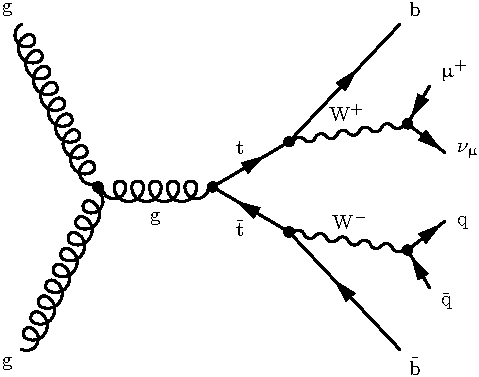
\includegraphics[width=0.4\textwidth]{assets/Feynman/semilep_mu_tt.pdf}
\caption[Semileptonic Decay of a Top Quark Pair]{\textbf{Semileptonic decay of a top quark pair.} The process is in LO of QCD in respect of the final state particles. To be unbiased of the selected jets, no selection for b jets is done. The quarks from the W boson decay are preferably light flavor or c quarks. The charged conjugated process is also possible.}
\label{fig:ch_6_semilep_mu}
\end{figure}

\subsection{Datasets}
The datasets for recorded events are sorted in respect of L1 triggers and the HLTs. The appropriate dataset for this selection is the single muon dataset. Each event was accepted by one or several HLTs of this category. For later steps, events are only taken if they passed one of two specific HLTs for isolated muons with $\pt > 24\GeV$. The use of a HLT selection on data and simulation ensures that no events from other datasets for data are represented in the simulated datasets. For the data, the recorded events from all periods of 2016 were taken. The total recorded luminosity is $\mathcal{L} = 35.14\,\textrm{fb}^{-1}$, it was computed using the \brilcalc \cite{brilcalc} tool.\\

The simulated events are sorted by the hard scattering process, additional jets can occur from pileup, initial or final state radiation or from the parton shower. The t$\bar{\textrm{t}}$ processes were generated by \powheg including NLO processes in QCD. For the W boson processes with additional jets, a dataset with NLO in QCD exists, this dataset is modeled with \amcatnlo and has negative lhe weights and the statistic is low. Alternative datasets exist in LO with more events. These are grouped in the number of jets in the final state of the hard process. The datasets for a W boson with two, three and four additional jets were taken. The Drell-Yan processes are generated with \amcatnlo and grouped in respect of the invariant mass $M_\textrm{inv}$ of the virtual photon or Z boson. Two datasets, one for $10\,\GeV < M_\textrm{inv} < 50\,\GeV$ and one for $M_\textrm{inv}>\,50\GeV$ were taken. The single t processes are grouped in respect of their production mode and generated with {\powheg}. The four main contributing production channels were taken, these are single top quark production in the t-channel and in association with an W boson and the corresponding processes for antitop quarks. The subsequent effects of all processes were modeled by \pythia 8 while the detector simulation is performed with {\geant}. The number of events and the cross section of each process are listed in table \ref{tab:ch_6_Datasets}.

\begin{table}[t]
\caption[Hard-Scattering Processes]{\textbf{Generated hard-scattering processes and their cross sections.} The higher the cross section $\sigma$ and the lower the number of generated events $N_{\textrm{gen}}$ is, the worse the statistic. One can see, the W + jets dataset has the worst statistic, in the semileptonic selection, it was chosen to take the jet grouped datasets instead. The processes where two bosons are involved have only a significant contribution in the dileptonic selection.}
\label{tab:ch_6_Datasets}
\begin{tabular}{lS[table-number-alignment = right]
					S[table-number-alignment = center,table-figures-decimal = 2]}
\toprule
{Dataset $\qquad$} & {$\qquad N_{\textrm{gen}}\qquad$} & {$\qquad\sigma$ in pb $\quad$} \\ 
\midrule
t$\bar{\textrm{t}}$ & 154948894 & 831.76 \cite{TopPP}\\
DY($10\,\GeV < M_\textrm{inv} < 50\,\GeV$) & 47946519 & 6025.2 \cite{DYCrossSec}\\
DY($M_\textrm{inv} > 50\,\GeV$) & 81781052 & 22635.1 \cite{DYCrossSec}\\
W + jets & 16497031 & 61526.7 \cite{DYCrossSec}\\
W + 2 jets & 29878415 & 3161 \cite{GenXSec}\\
W + 3 jets & 19798117 & 948.2 \cite{GenXSec} \\
W + 4 jets & 9170576 & 494.6 \cite{GenXSec}\\
single t (t-channel) & 67240808 & 136.02 \cite{HatHor1,HatHor2}\\
single $\bar{\textrm{t}}$ (t-channel) & 38811017 & 80.95 \cite{HatHor1,HatHor2}\\
Wt & 6952830 & 35.6 \cite{HatHor1,HatHor2}\\
W$\bar{\textrm{t}}$ & 6933094 & 35.6 \cite{HatHor1,HatHor2}\\
WW & 994012 & 118.7 \cite{BosonPairCrossSec}\\
WZ & 1000000 & 44.9 \cite{BosonPairCrossSec}\\
ZZ & 998034 & 15.4 \cite{BosonPairCrossSec}\\
\bottomrule
\end{tabular}
\end{table}

\subsection{Data-to-Simulation Comparison}
To compare the data with the simulation, the events from the simulation of a certain process $i$ have to be scaled, this is done by assigning a weight for each event depending on the process. The weight is determined by the corresponding cross section $\sigma_i$ and the efficiency $\epsilon_i$. The $\epsilon_i$ is the number of selected events divided by the number of generated events $N_{i,\textrm{gen}}$. The events have also to be scaled with the luminosity of the data that is in comparison. Each event of the simulation gets an event weight of
\begin{equation}
w_i = \mathcal{L} \frac{ \sigma_i}{N_{i,\textrm{gen}}} \quad . 
\end{equation}
The $\epsilon_i$ results from summing up all events. Further improvements can be achieved by applying reweighting for each event depending on known scalefactors, this was discribed in section \ref{sec:ch_3_Reweighting}. In this selection, scalefactors were applied for the tight muon ID ($sf^\textrm{ID}$), for the muon isolation ($sf^\textrm{Iso}$), for the muon efficiency in the tracker ($sf^\textrm{Track}$) and for the HLT selection ($sf^\textrm{HLT}$). These depend on the muon \pt and $\eta$ value. Furthermore, a pileup reweighting $w_\textrm{PU}$ was performed, depending on the number of PV of each event. Additionally one has to take negative event weights $w_\textrm{lhe}$ for events generated with the \amcatnlo matrix element generator into account (as explained in section \ref{sec:ch_3_simtools}). These appear in Drell-Yan processes. For this dataset, one has to compute an effective number of generated events $N_{i,\textrm{gen}}^\textrm{eff}$, which is the number of events with positive weights subtracted by the number of events with negative weights. The scalefactors are different for the various periods of the total run 2 in 2016. Therefore, they have to be weighted with the corresponding luminosity. The event weight for each event is then given by
\begin{equation}
\begin{split}
w_i(nPV,&\pt,\eta, w_\textrm{lhe}) = \frac{\sigma_i}{N_{i,\textrm{gen}}^\textrm{eff}}\cdot w^\textrm{PU}(nPV) \cdot w_\textrm{lhe} \\
 & \cdot \sum_{r \in \{\textrm{Periods}\}} \mathcal{L}_r \cdot sf^\textrm{ID}_r(\pt,\eta) \cdot sf^\textrm{Iso}_r(\pt,\eta) \cdot sf^\textrm{Track}_r(\eta) \cdot sf^\textrm{HLT}_r(\pt,\eta) 
\end{split}
\end{equation}
The data to simulation agreement can be investigated by looking at distributions of different variables. Four meaningful variables are shown in figure \ref{fig:ch_6_semilepDist}. The fact that the number of events in simulation is lower than in data is a hint for an additional process which was not included here. This could be QCD processes, however QCD processes are more complicated to implement. Since the shape is in a good agreement, and this is the more important fact, the selection is sufficient for the domain adaptation studies.


\begin{figure}[!ht]
   \begin{minipage}{\textwidth}
     \centering
     \subfigure[]{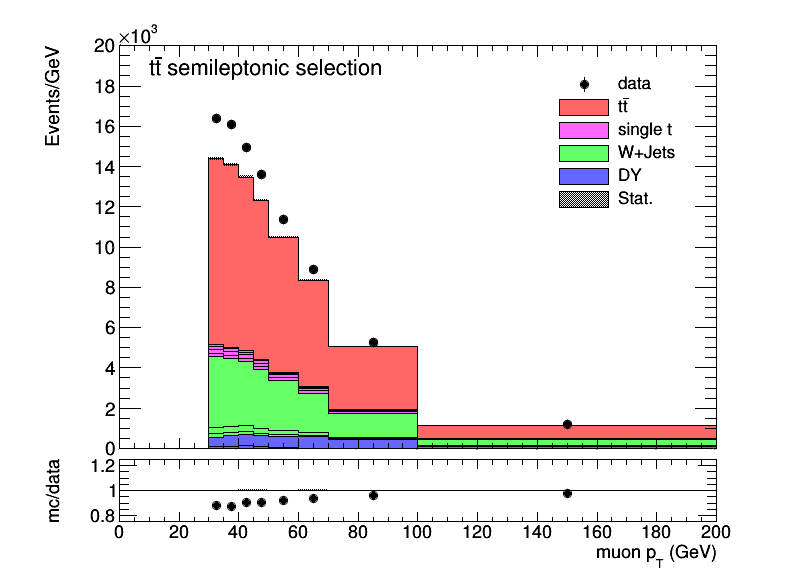
\includegraphics[width=7cm]{assets/semilep_pt.png}}\quad
     \subfigure[]{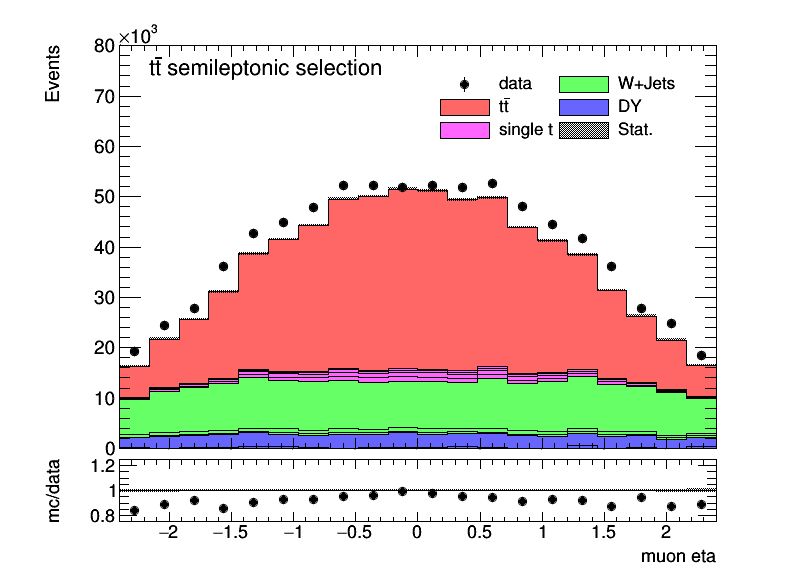
\includegraphics[width=7cm]{assets/semilep_eta.png}}\\
     \subfigure[]{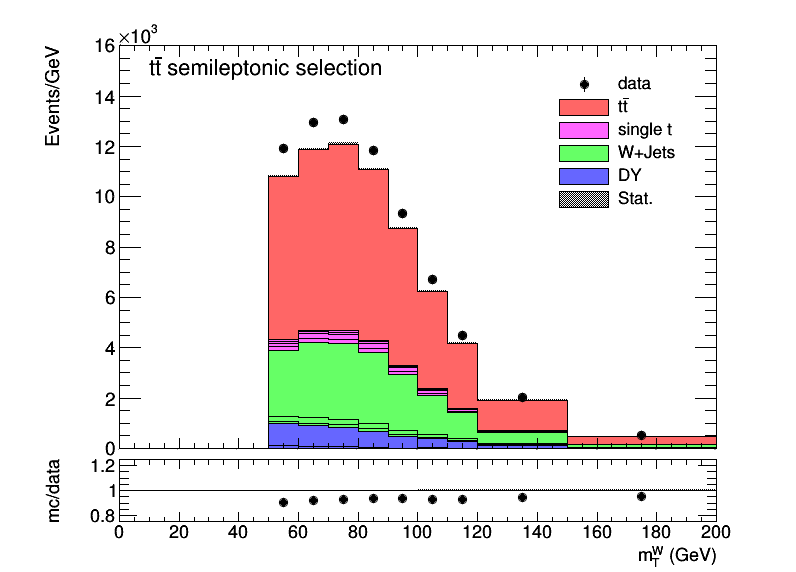
\includegraphics[width=7cm]{assets/semilep_mwt.png}}\quad
     \subfigure[]{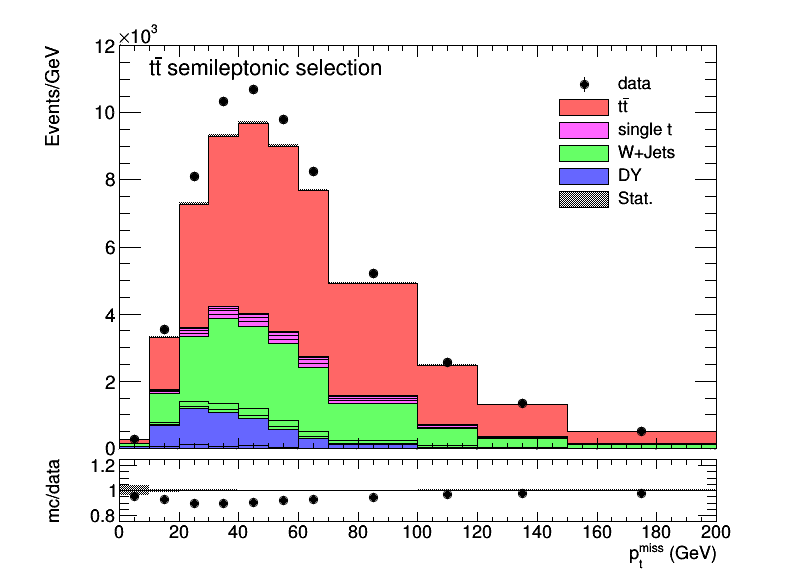
\includegraphics[width=7cm]{assets/semilep_ptmiss.png}}
     
   \end{minipage}\\[1em]
	\caption[Distributions of Variables from the Semileptonic Selection]{\textbf{Distributions of variables from the semileptonic selection.} Shown are the distributions of muon \pt (a), muon $\eta$ (b), reconstructed transverse energy of the W boson $m^\textrm{W}_\textrm{T}$ (c) and the missing transverse energy $\pt^\textrm{miss}$ (d). The total amount of events in data is about 7 \% higher compared to the simulation. The shape in each distribution is in good agreement. The statistic uncertainties are negligible, systematic uncertainties have not been computed.}
	\label{fig:ch_6_semilepDist}
\end{figure}


\section{Top Quark Pair - Dileptonic  Selection} \label{sec:ch_6_dilep}
The dileptonic decay mode can be further distinguished in respect of the leptons in the final state. The decay mode with two muons or two electrons in the final state are dominated by Drell-Yan processes which have mainly additional light flavor quark and gluon jets. The decay mode with a muon and an electron with opposite charge, shown in figure \ref{fig:ch_6_semilep_dilep} has the clearest signal for t$\bar{\textrm{t}}$ and is therefore preferred. The selection criteria are
\begin{description}
\setlength{\itemsep}{-20pt}
\item[•] one good muon with \pt > 20,\\
\item[•] one good electron with opposite charge,\\
\item[•] $M_\textrm{inv} > 20\,\GeV$ of the electron-muon pair to reject backgrounds,\\
\item[•] the good electron or the good muon with $\pt > 25\,\GeV$,\\
\item[•] a trigger selection, which is explained in the following.
\end{description}
The main contributions from other processes are Drell-Yan processes where, for example one muon is misidentified as an electron. Minor contributions coming from vector boson pairs (WW, WZ and ZZ), W boson processes and single top quark processes. 

\begin{figure}
\centering
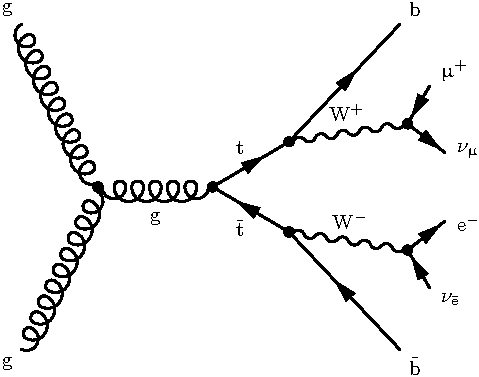
\includegraphics[width=0.4\textwidth]{assets/Feynman/dilep_emu_tt.pdf}
\caption[Dileptonic Decay of a Top Quark Pair]{\textbf{Dileptonic decay of a top quark pair.} With a selection of the muon and electron, a high fraction of t$\bar{\textrm{t}}$ events can be achieved, and therefore many b jets are obtained. Further cuts on the amount of jets or the missing $p_\textrm{T}^\textrm{miss}$ are not necessary for this thesis. Additional jets through initial or final state radiation, pileup or through the parton shower are possible.}
\label{fig:ch_6_semilep_dilep}
\end{figure}

\subsection{Datasets}
The measured events are taken from the muon-electron/photon dataset. Two HLTs were used in the selection where both require one isolated muon and one isolated electron. The first (second) has a limit for the muon of $\pt > 23\,\GeV$ ($\pt > 8\,\GeV$) and for the electron of $\pt > 12\,\GeV$ ($\pt > 23\,\GeV$). Unfortunately there was a problem during the periods of 2016, two different pairs of these HLTs were used. The total recorded luminosity for this dataset was again computed using the \brilcalc tool to a value of $\mathcal{L} = 35.199\,\textrm{fb}^{-1}$.\\

For the simulation, the same datasets were used for the t$\bar{\textrm{t}}$, Drell-Yan, Wt, and W$\bar{\textrm{t}}$ processes. For the W boson with additional jets, the W + jets datasets was used here. Single t and single $\bar{\textrm{t}}$ processes in the t-channel have a negligible contribution and are not included. Instead, processes with two bosons were included, the \pythia 8 program were used for the matrix element generation in NLO and the simulation of subsequent processes. The datasets are given in table \ref{tab:ch_6_Datasets}. 

\subsection{Data-to-Simulation Comparison}
The comparison was done in the same way than for the semileptonic selection in the last section. The fact that two different sets of trigger were used during the periods of the 2016 data has to be taken into account for the simulation. The event weights are therefore additionally multiplied with a flag $f \in \{0,1\}$ of the HLT of the corresponding period. Moreover a trigger for the isolated electron $sf^\textrm{IDandISO}$ has to be included. The event weight is then given by
\begin{equation}
\begin{split}
w_i(nPV,\, p_{\textrm{T},\upmu},\, \eta_\upmu,\, p_\textrm{T,el},\, \eta_\textrm{el},\, &\eta_\textrm{SC,el},\, w_\textrm{lhe},\, f_r) = \frac{\sigma_i}{N_{i,\textrm{gen}}^\textrm{eff}} \cdot w^\textrm{PU}(nPV) \cdot w_\textrm{lhe}\\
 \cdot \sum_{r \in \{\textrm{Periods}\}} \biggl( f_r  \cdot \mathcal{L}_r \cdot &sf^\textrm{ID}_r(p_{\textrm{T},\upmu},\eta_\upmu) \cdot sf^\textrm{Iso}_r(p_{\textrm{T},\upmu},\eta_\upmu) \cdot sf^\textrm{Track}_r(\eta_\upmu)  \\
  \cdot &sf^\textrm{IDandISO}_r(p_\textrm{T,el},\eta_\textrm{SC,el}) \cdot sf^\textrm{HLT}_r(\eta_\textrm{el},\eta_\upmu) \biggr)
\end{split}
\end{equation}
The selection has no requirement of the number of jets. The number of jets together with distributions for the leading (trailing) lepton, which is the good muon or good electron with the highest (lowest) {\pt}, is shown in figure \ref{fig:ch_6_dilepDist}. 



\begin{figure}[!ht]
   \begin{minipage}{\textwidth}
     \centering
     \subfigure[]{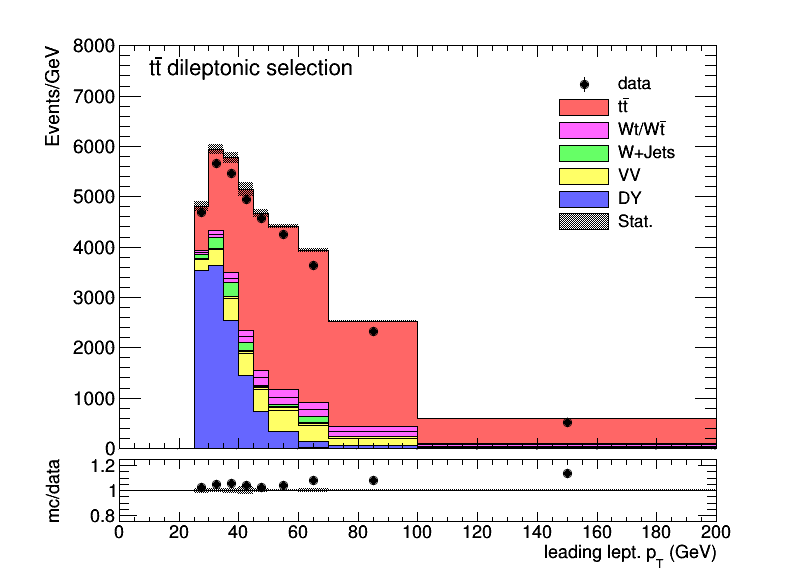
\includegraphics[width=7cm]{assets/dilep_ll_pt.png}}\quad
     \subfigure[]{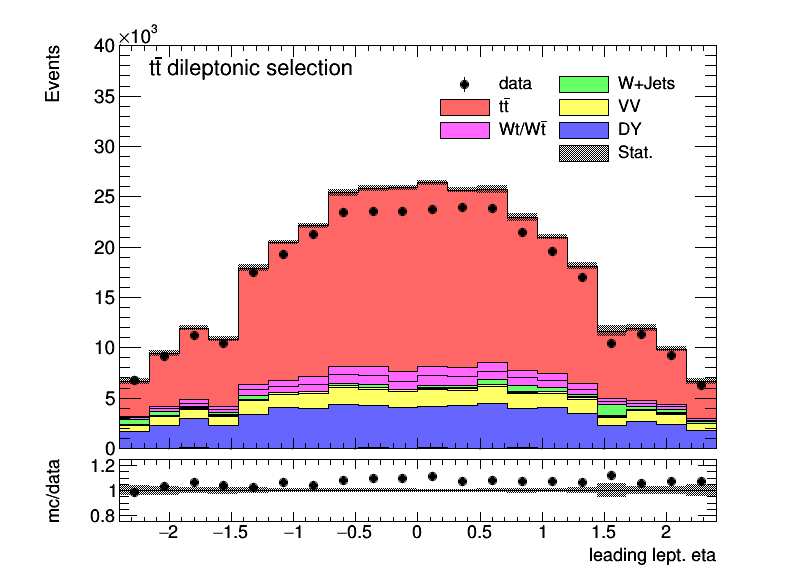
\includegraphics[width=7cm]{assets/dilep_ll_eta.png}}\\
     \subfigure[]{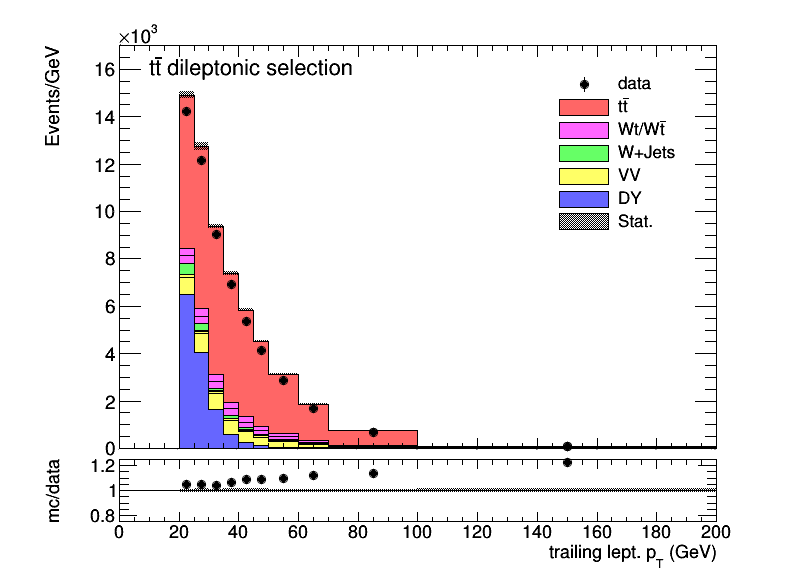
\includegraphics[width=7cm]{assets/dilep_tl_pt.png}}\quad
     \subfigure[]{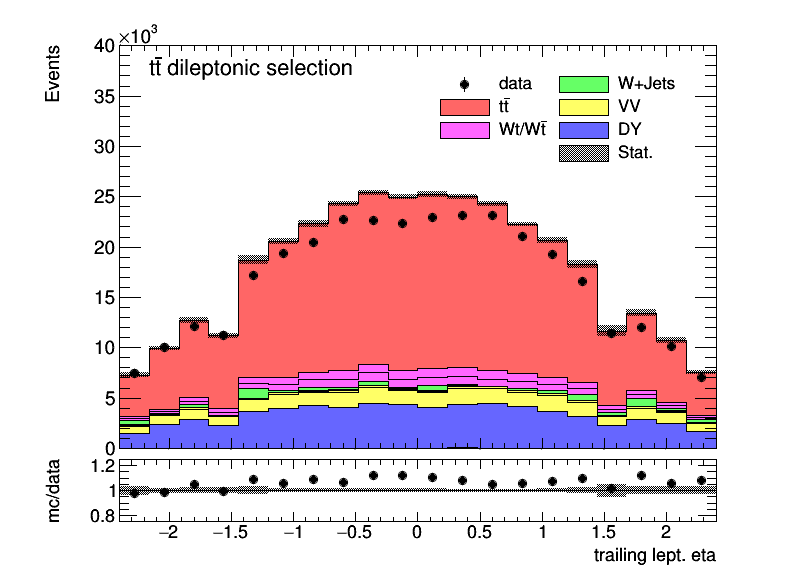
\includegraphics[width=7cm]{assets/dilep_tl_eta.png}}\\
     \subfigure[]{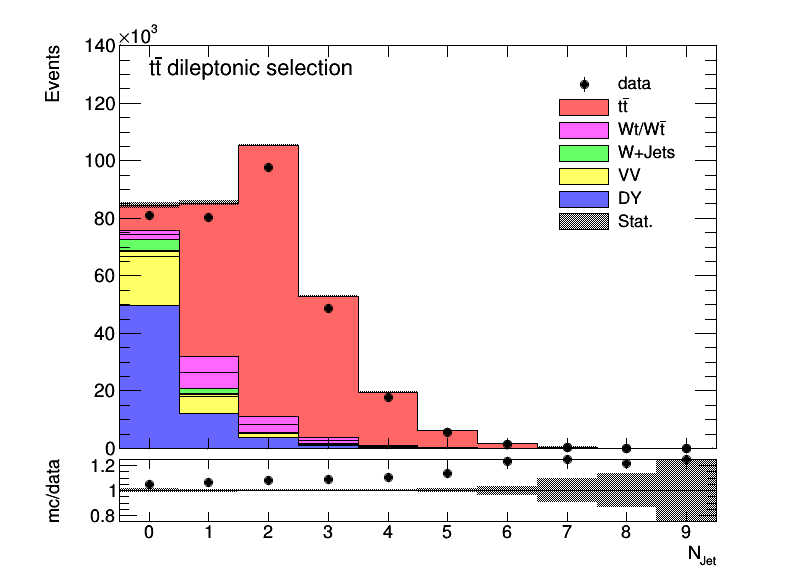
\includegraphics[width=7cm]{assets/dilep_njets.png}}
     
   \end{minipage}\\[1em]
	\caption[Distributions of Variables from the Dileptonic Selection]{\textbf{Distributions of variables from the dileptonic selection.} Shown are the distributions of \pt (a) and $\eta$ (b) of the leading lepton, and the \pt (c) and $\eta$ (d) of the trailing lepton and the number of jets (e) in each event. The number of simulated events is about 7 \% higher than the number of events in data. The reason is assumed in wrong scalefactors. However the shape is again in a good agreement. The statistical uncertainties are higher but still negligible, the systematic uncertainties are not given.}
	\label{fig:ch_6_dilepDist}
\end{figure}
